\documentclass[tikz,border=12pt]{standalone}
\usepackage[utf8]{inputenc}
\usepackage{tikz}
\usetikzlibrary{shapes,arrows.meta,positioning,calc}

\definecolor{ScoutGreen}{HTML}{005432}
\definecolor{ScoutNavy}{HTML}{002855}
\definecolor{ScoutBlue}{HTML}{006EB6}
\definecolor{ScoutRed}{HTML}{A31920}
\definecolor{ScoutAmber}{HTML}{D97706}
\definecolor{BorderGray}{HTML}{CBD5E1}

\begin{document}
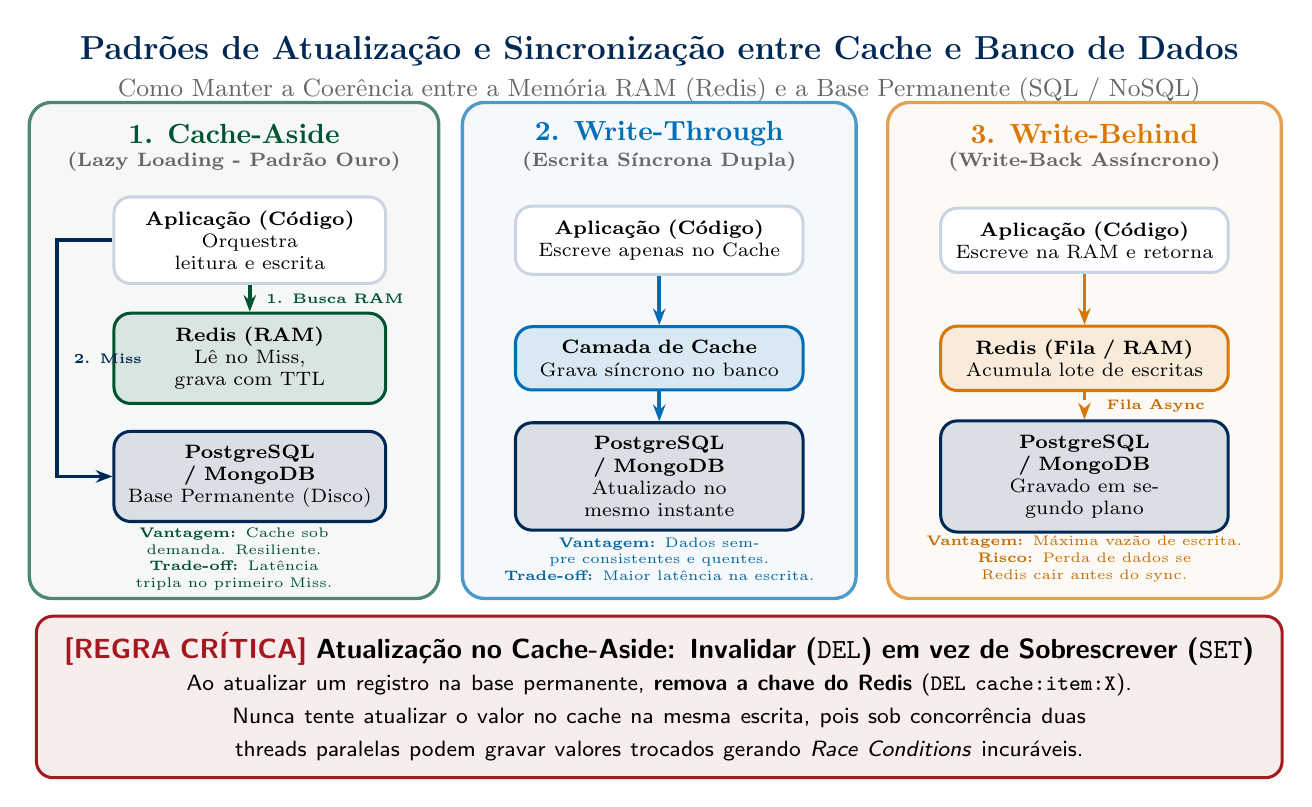
\begin{tikzpicture}[
    font=\sffamily,
    box/.style={draw=BorderGray, rounded corners=6pt, fill=white, line width=1.1pt, align=center, inner sep=5pt},
    arrow/.style={-{Stealth[length=6pt]}, line width=1.3pt}
]

  % Título Geral
  \node[font=\bfseries\large, text=ScoutNavy] at (8.0, 7.6) {Padrões de Atualização e Sincronização entre Cache e Banco de Dados};
  \node[font=\small, text=gray!80!black] at (8.0, 7.1) {Como Manter a Coerência entre a Memória RAM (Redis) e a Base Permanente (SQL / NoSQL)};

  % =========================================================================
  % PADRÃO 1: CACHE-ASIDE (LAZY LOADING)
  % =========================================================================
  \node[draw=ScoutGreen!70, rounded corners=8pt, fill=ScoutGreen!4, line width=1.2pt, minimum width=5.2cm, minimum height=6.3cm] (p1) at (2.6, 3.8) {};
  \node[font=\bfseries\normalsize, text=ScoutGreen] at (2.6, 6.55) {1. Cache-Aside};
  \node[font=\scriptsize\bfseries, text=gray!80!black] at (2.6, 6.2) {(Lazy Loading - Padrão Ouro)};

  \node[box, text width=3.1cm, font=\scriptsize] (c1_app) at (2.8, 5.2) {\textbf{Aplicação (Código)}\\Orquestra leitura e escrita};
  \node[box, fill=ScoutGreen!15, draw=ScoutGreen, text width=3.1cm, font=\scriptsize] (c1_cache) at (2.8, 3.7) {\textbf{Redis (RAM)}\\Lê no Miss, grava com TTL};
  \node[box, fill=ScoutNavy!15, draw=ScoutNavy, text width=3.1cm, font=\scriptsize] (c1_db) at (2.8, 2.2) {\textbf{PostgreSQL / MongoDB}\\Base Permanente (Disco)};

  \draw[arrow, color=ScoutGreen] (c1_app) -- node[right=2pt, font=\tiny\bfseries, text=ScoutGreen] {1. Busca RAM} (c1_cache);
  \draw[arrow, color=ScoutNavy] (c1_app.west) -- ++(-0.7, 0) |- node[pos=0.25, right=2pt, font=\tiny\bfseries, text=ScoutNavy] {2. Miss} (c1_db.west);

  \node[font=\tiny, text=ScoutGreen!90!black, align=center, text width=4.5cm] at (2.6, 1.15) {
    \textbf{Vantagem:} Cache sob demanda. Resiliente.\\\textbf{Trade-off:} Latência tripla no primeiro Miss.
  };

  % =========================================================================
  % PADRÃO 2: WRITE-THROUGH
  % =========================================================================
  \node[draw=ScoutBlue!70, rounded corners=8pt, fill=ScoutBlue!4, line width=1.2pt, minimum width=5.0cm, minimum height=6.3cm] (p2) at (8.0, 3.8) {};
  \node[font=\bfseries\normalsize, text=ScoutBlue] at (8.0, 6.55) {2. Write-Through};
  \node[font=\scriptsize\bfseries, text=gray!80!black] at (8.0, 6.2) {(Escrita Síncrona Dupla)};

  \node[box, text width=3.3cm, font=\scriptsize] (c2_app) at (8.0, 5.2) {\textbf{Aplicação (Código)}\\Escreve apenas no Cache};
  \node[box, fill=ScoutBlue!15, draw=ScoutBlue, text width=3.3cm, font=\scriptsize] (c2_cache) at (8.0, 3.7) {\textbf{Camada de Cache}\\Grava síncrono no banco};
  \node[box, fill=ScoutNavy!15, draw=ScoutNavy, text width=3.3cm, font=\scriptsize] (c2_db) at (8.0, 2.2) {\textbf{PostgreSQL / MongoDB}\\Atualizado no mesmo instante};

  \draw[arrow, color=ScoutBlue] (c2_app) -- (c2_cache);
  \draw[arrow, color=ScoutBlue] (c2_cache) -- (c2_db);

  \node[font=\tiny, text=ScoutBlue!90!black, align=center, text width=4.5cm] at (8.0, 1.15) {
    \textbf{Vantagem:} Dados sempre consistentes e quentes.\\\textbf{Trade-off:} Maior latência na escrita.
  };

  % =========================================================================
  % PADRÃO 3: WRITE-BEHIND (WRITE-BACK)
  % =========================================================================
  \node[draw=ScoutAmber!70, rounded corners=8pt, fill=ScoutAmber!4, line width=1.2pt, minimum width=5.0cm, minimum height=6.3cm] (p3) at (13.4, 3.8) {};
  \node[font=\bfseries\normalsize, text=ScoutAmber] at (13.4, 6.55) {3. Write-Behind};
  \node[font=\scriptsize\bfseries, text=gray!80!black] at (13.4, 6.2) {(Write-Back Assíncrono)};

  \node[box, text width=3.3cm, font=\scriptsize] (c3_app) at (13.4, 5.2) {\textbf{Aplicação (Código)}\\Escreve na RAM e retorna};
  \node[box, fill=ScoutAmber!15, draw=ScoutAmber, text width=3.3cm, font=\scriptsize] (c3_cache) at (13.4, 3.7) {\textbf{Redis (Fila / RAM)}\\Acumula lote de escritas};
  \node[box, fill=ScoutNavy!15, draw=ScoutNavy, text width=3.3cm, font=\scriptsize] (c3_db) at (13.4, 2.2) {\textbf{PostgreSQL / MongoDB}\\Gravado em segundo plano};

  \draw[arrow, color=ScoutAmber] (c3_app) -- (c3_cache);
  \draw[arrow, color=ScoutAmber, dashed] (c3_cache) -- node[right=4pt, font=\tiny\bfseries, text=ScoutAmber!90!black] {Fila Async} (c3_db);

  \node[font=\tiny, text=ScoutAmber!90!black, align=center, text width=4.5cm] at (13.4, 1.15) {
    \textbf{Vantagem:} Máxima vazão de escrita.\\\textbf{Risco:} Perda de dados se Redis cair antes do sync.
  };

  % =========================================================================
  % REGRA DE OURO DA ATUALIZAÇÃO
  % =========================================================================
  \node[draw=ScoutRed, fill=ScoutRed!8, rounded corners=6pt, text width=15.4cm, align=center, line width=1.1pt, inner sep=6pt] at (8.0, -0.6) {
    \textbf{\textcolor{ScoutRed}{[REGRA CRÍTICA]} Atualização no Cache-Aside: Invalidar (\texttt{DEL}) em vez de Sobrescrever (\texttt{SET})}\\[2pt]
    \footnotesize Ao atualizar um registro na base permanente, \textbf{remova a chave do Redis} (\texttt{DEL cache:item:X}).\\
    Nunca tente atualizar o valor no cache na mesma escrita, pois sob concorrência duas threads paralelas podem gravar valores trocados gerando \textit{Race Conditions} incuráveis.
  };

\end{tikzpicture}
\end{document}
